\subsubsection{振る舞い設計記述}

\term{振る舞い設計記述}{Behavioral Design Description} は、ソフトウェアが時間の中でどのように動くかを表す。処理の流れ、イベントへの反応、状態変化、入力と出力の関係などを示す。

代表的な記法は次のとおりである。

\par\smallskip\noindent\refstepcounter{table}\label{tab:ch03-05}\textbf{表 \thetable: 第03章 ソフトウェア設計 表05}\par\smallskip
\begin{longtable}{L{42mm}L{112mm}}
\toprule
\textbf{記法} & \textbf{説明} \\
\midrule
\endhead
活動図 & 処理の流れ、分岐、並行活動、入力、出力を表す。 \\
相互作用図 & オブジェクトや構成要素間のメッセージ交換を表す。通信図とシーケンス図が代表である。 \\
データフロー図 & 処理要素間を流れるデータを表す。セキュリティ分析にも使える。 \\
決定表・決定図 & 条件の組合せと、それに対応する動作を表す。複雑な業務規則に向く。 \\
フローチャート & 制御の流れと処理順序を表す。 \\
状態遷移図・状態チャート & 状態、イベント、遷移、状態ごとの振る舞いを表す。 \\
形式仕様言語 & 数学的な記法で、インタフェースや振る舞いを厳密に定義する。 \\
擬似コード・プログラム設計言語 & プログラムに近い形で処理手順を表す。詳細設計やアルゴリズム説明に使う。 \\
\bottomrule
\end{longtable}

\begin{figure}[htbp]
\centering
\IfFileExists{assets/fig-ch03-08.png}{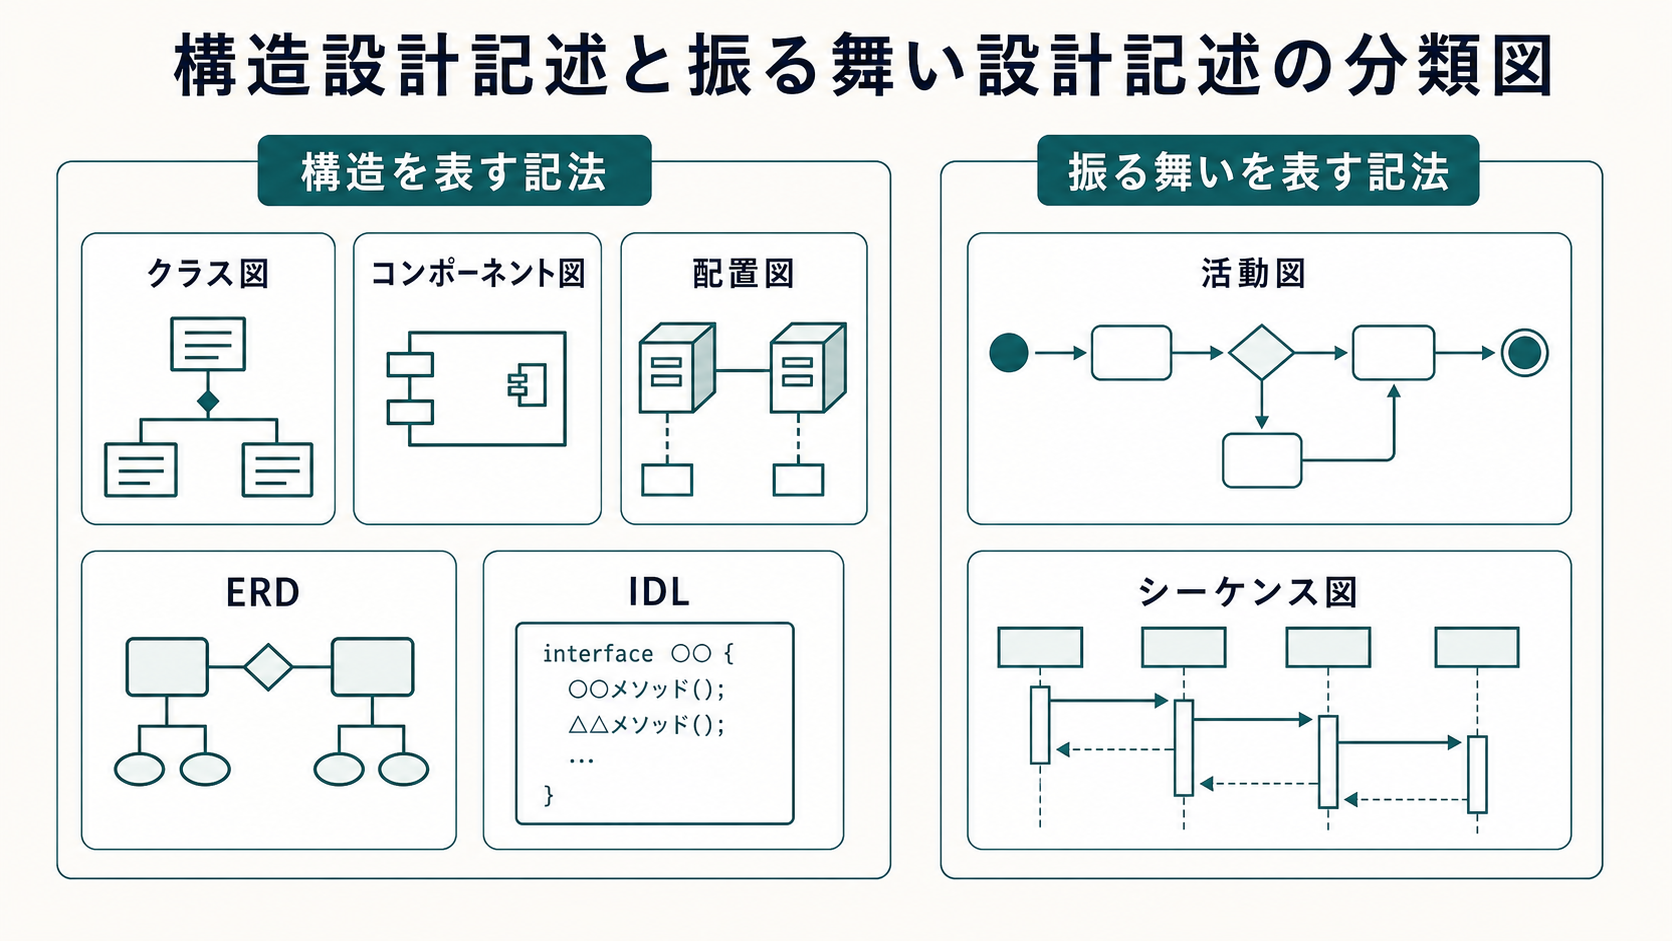
\includegraphics[width=0.96\linewidth]{assets/fig-ch03-08.png}}{\fbox{\parbox[c][48mm][c]{0.9\linewidth}{\centering 画像生成待ち\\構造設計記述と振る舞い設計記述の分類図}}}
\caption{構造設計記述と振る舞い設計記述の分類図}
\label{fig:ch03-08}
\end{figure}
